\section{Evaluation}\label{sec:eval}

We ask four research questions. 
(1) Do coupled decisions make urban sorties safer and more productive than the decoupled practice
of today (Sect.~\ref{sec:eval:overall})? 
(2) Which coupling is responsible for which part of the gain (Sect.~\ref{sec:eval:ablation})? 
(3) What does the coupling cost, and does the runtime keep it inside the real-time budget
of a fleet (Sect.~\ref{sec:eval:micro})? 
(4) Can operators reach the runtime from ordinary devices without a server GPU (Sect.~\ref{sec:eval:access})? 
We then test how sensitive the results are to the decision parameters
(Sect.~\ref{sec:eval:sens}) and whether the shared model is in fact the same model everywhere
(Sect.~\ref{sec:eval:consistency}).

\subsection{Setup}\label{sec:eval:setup}

Table~\ref{tab:config} summarises the configuration. All campaigns run the complete runtime of Sect.~\ref{sec:design}
in-process with a simulated clock that advances faster than real time; only the decision-awareness switches differ
between policies, and the simulated ground truth (wind acting on the dynamics, contact with the surface model, battery
discharge) is always fully coupled. A sortie is \emph{completed} if the drone lands within 25\,m of its depot,
\emph{lost} if it collides with a building or the ground or ends away from home with an empty battery, \emph{returned
early} if the battery logic recalls it before its station time ends, and \emph{not launched} if the precheck refuses
it. We call a sortie \emph{unsafe} if it is lost or if it is launched although the field wind along its route exceeds
the vehicle's 13.8\,m/s rating. Intervals are 95\% percentile bootstrap intervals; for closed-loop campaigns the bootstrap resamples whole
tasks (city, weather and seed), because the sorties of one task share their conditions. Large language models were used
to help search the literature and edit the text and to produce simulated reviewer critiques of a draft; they did not
generate, select or analyse any experimental data.

\begin{table}[t]
\caption{Experiment configuration.}\label{tab:config}
\footnotesize
\begin{tabularx}{\textwidth}{@{}lX@{}}
\toprule
Server & 64-core Intel Xeon Gold 6426Y, 503\,GB RAM, Linux 6.8, Python 3.12; no GPU used by the runtime \\
Clients & Apple M3 laptop (Chrome, Metal); headless Chromium on the server with SwiftShader (software) and with an NVIDIA A100 (Vulkan) \\
Cities & Shenzhen, Shanghai, Suzhou, New York, Chicago, San Francisco (UrbanScene3D~\cite{lin2022urbanscene3d}) and SynthCity (procedural, 1.2\,km) \\
Weather & the 12 presets of the environment field, from clear to thunderstorm; wind direction drawn per seed \\
Vehicle & P600-class hexacopter reference model: 222\,Wh battery, 85\% usable, 20\% launch reserve, wind rating 13.8\,m/s \\
Return campaign & 8 drones per task, on-station points at 40\,m above ground 300--1,100\,m from the depot, station time 30--300\,s, \RTLSEEDS{} seeds per city and preset, 9 policies (\RTLSORTIES{} sorties) \\
Scan campaign & 500\,m area of interest, 400 standing persons on open ground, detection, recognition and identification plans, 3 seeds per city and preset, plus a MOR sweep from 100\,m to 5\,km \\
Front campaign & sorties as above launched in clear air while the weather turns into rain, heavy rain or a thunderstorm over 10\,min; 5 seeds per city and front; PX4 default, snapshot and space-time precheck \\
Delegation & 12 drones (half with a 4.8--48\,mm zoom, half with a fixed 4.8\,mm lens), state of charge 12--90\%, 30 observation requests per task, 5 seeds per city and preset \\
Policies & PX4 default return (climb to 30\,m above home, straight line, battery thresholds) without mission precheck; a decoupled stack (wind-blind energy precheck, geometry- and wind-blind return); the coupled policy; and one ablation per coupling. Scan: weather-blind plan sized for clear air vs coupled plan. Delegation: nearest drone, contract net with clear-air perception quotes, and coupled contract net \\
\bottomrule
\end{tabularx}
\end{table}

\subsection{Overall performance}\label{sec:eval:overall}

\paragraph{Launch and return.} Figure~\ref{fig:overall-heatmap} shows, for every city and weather preset, the share of
sorties that end unsafe under the PX4 default and under the coupled policy, and the share the coupled policy completes.
Under the PX4 default, \PXUNSAFE\% of all sorties are unsafe: in calm and wet weather most of them are returns that fly
into buildings, between \PXCITYLO\% of sorties in \PXCITYLOW{} and \PXCITYHI\% in \PXCITYHIW{}, and in severe weather every launched
sortie flies beyond the wind rating. The coupled policy reduces the unsafe share to \CPUNSAFE\% and at the same time
completes \CPDONE\% of sorties instead of \PXDONE\%. Of its 34 residual collisions, 30 occur on one pad of the San
Francisco depot, within one metre of the pad at lift-off or touchdown, and the same sorties collide under the other
policies as well; they are a property of that pad cell in the surface model rather than of a decision. The other four
are collisions between two returning drones in SynthCity, which the separation layer, not the return planner, has to
resolve. The decoupled stack, which adds a wind-blind energy precheck to a geometry-
and wind-blind return, behaves like the PX4 default (\DCUNSAFE\% unsafe, \DCDONE\% completed): an energy precheck
alone does not help when the return it budgets for is the wrong one.

\begin{figure}[t]
\centering
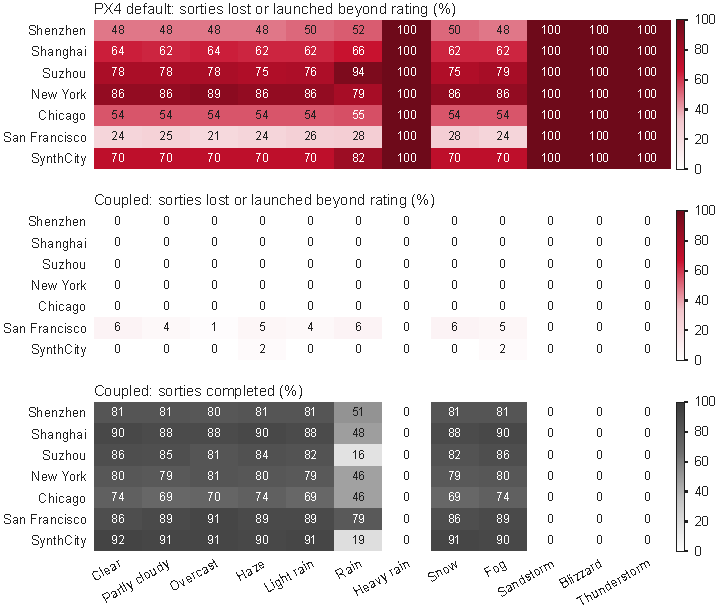
\includegraphics[width=\textwidth]{figures/pdf/overall_heatmap.pdf}
\caption{Overall performance per city and weather preset (\RTLSEEDS{} seeds, 8 sorties each). Top: sorties lost or
launched beyond the wind rating under the PX4 default. Middle: the same under the coupled policy. Bottom: sorties the
coupled policy completes. Presets in which the field wind exceeds the rating are not launched by the coupled policy}
\label{fig:overall-heatmap}
\end{figure}

Figure~\ref{fig:overall-outcomes}a breaks the outcomes down by weather group. In calm weather the coupled policy
completes \CPCALMDONE\% of sorties against \PXCALMDONE\% for the PX4 default, because the PX4 default loses \PXCALMLOST\% of its sorties on the
way home; the coupled policy declines \CPCALMDECL\% of the calm-weather sorties, whose cruise altitude over the
buildings is about twice that of the launched ones and whose mission energy would break the launch reserve. In wet and windy weather the coupled policy declines \CPWETDECL\% of the sorties, those whose route wind
exceeds the rating or whose return under the field wind would break the reserve, and completes \CPWETDONE\%; the PX4 default
launches all of them, completes \PXWETDONE\% and flies \PXWETOVER\% beyond the rating. In severe weather the coupled policy launches
nothing, while the PX4 default loses \PXSEVLOST\% of its sorties. Declining is the honest answer in these cases, and the
precheck reports it before take-off instead of discovering it in flight.

Where does the safety come from? Figure~\ref{fig:overall-outcomes}b shows how high the returns climb above the depot.
The PX4 default returns at the higher of its current altitude and 30\,m above home, so a drone on station 40\,m above
the ground flies home at about its station altitude (median \PXCLIMB\,m above the depot), and collides on
\PXCOLL\% of sorties. Climbing over the highest point of the clearance envelope on the return line removes the collisions
but makes the median return climb \NDCLIMB\,m. The coupled policy keeps the same collision rate with a median climb of
\CPCLIMB\,m, because detours around tall buildings replace the largest climbs, and spends \CPRETWH\,Wh per return against
\NDRETWH\,Wh.

\begin{figure}[t]
\centering
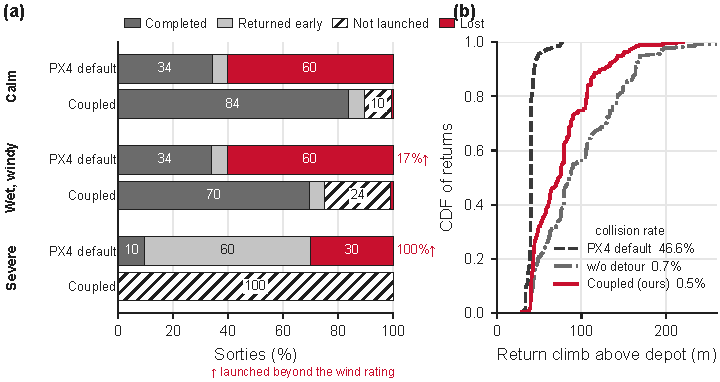
\includegraphics[width=\textwidth]{figures/pdf/overall_outcomes.pdf}
\caption{Outcome of every sortie. (a) Outcome shares per weather group; numbers with an upward arrow to the right are the sorties
launched beyond the wind rating. (b) Distribution of the return climb above the depot, with each policy's collision
rate over all sorties}
\label{fig:overall-outcomes}
\end{figure}

\paragraph{Weather fronts.} The campaigns above hold the weather constant. To test the time dimension of the shared
model, we launch the same sorties in clear air while the field holds a front that turns the weather into rain, heavy
rain or a thunderstorm over the next 10 minutes (7 cities, 5 seeds, 840 sorties per policy and front). Because the
transition is part of the field's keyframe, the space-time precheck of Sect.~\ref{sec:design:decisions} can query it
at the times the legs will be flown, while the snapshot precheck of the coupled policy sees only the clear air at
launch. We record the largest field wind at each drone's position during the flight and call a sortie unsafe if it is
lost or meets wind beyond the rating (Fig.~\ref{fig:front}). The snapshot precheck launches nearly every sortie into
the front: 40\%, 85\% and 89\% of its sorties are unsafe, and in the thunderstorm it loses 49\% of its sorties, 104 of the 137 lost in
emergency landings away from home once the drone can no longer hold its position. The PX4 default is worse still (65\%,
94\%, 96\%). The space-time precheck reduces the unsafe share to 11\%, 8\% and 4\%: it shortens the station time of
60--76\% of the sorties it launches into heavy rain and thunderstorms, to about two thirds of the request, and declines
those that cannot be back before the front. It delivers more safe station time than either alternative in heavy rain
and thunderstorms, and 11 points less than the snapshot precheck in rain, where its route wind, sampled at the cruise
altitude, is conservative. The precheck samples the route wind at three points of each leg; its remaining unsafe
sorties met stronger wind elsewhere on the path they actually flew.

\begin{figure}[t]
\centering
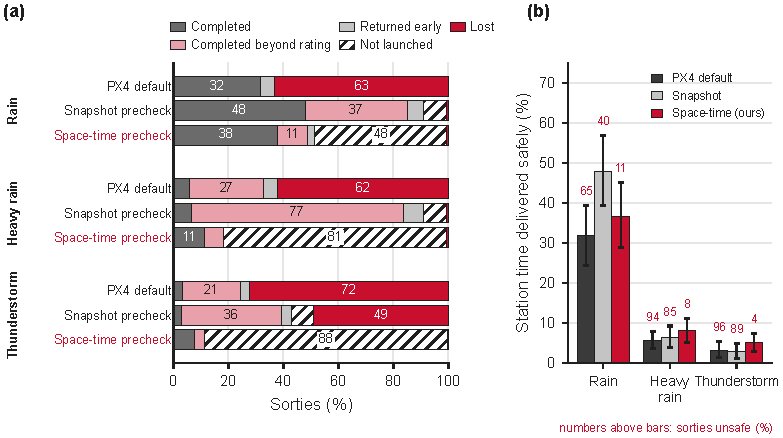
\includegraphics[width=\textwidth]{figures/pdf/front.pdf}
\caption{Weather fronts: sorties launched in clear air while a front builds over 10 minutes. (a) Outcome of every
sortie; ``completed beyond rating'' sorties came home but met field wind beyond the 13.8\,m/s rating. (b) Station
time delivered by sorties that came home within the rating, as a share of the requested station time; the numbers above the bars
are the unsafe sorties (lost or beyond the rating). Bars show 95\% task-level bootstrap intervals}
\label{fig:front}
\end{figure}

\paragraph{Scan planning.} Figure~\ref{fig:coverage-eval} evaluates the perception-driven scan planner of
Sect.~\ref{sec:design:decisions} in the three presets that reduce visibility. A weather-blind plan sized for clear air
captures 34\% of targets at detection level in fog and 5\% at recognition and identification level, and almost none in
a blizzard. The coupled planner flies lower and narrower strips under the field's optical depth and captures 82--91\%,
within a few points of the clear-air ceiling set by building occlusion. In a sandstorm, where visibility is reduced
less, the blind plan only loses recognition capture (73\% vs 89\%). The coupled plan reports the price of this capture
before launch: 1.34--1.41 times as many drones for recognition and identification and 1.05--1.27 times the makespan
(Fig.~\ref{fig:coverage-eval}b). In every other preset the two plans coincide, so the coupling costs nothing when the
weather does not matter. Planners that see only one of the two inputs separate their roles: a plan that knows the
visibility but not the wind captures as much as the coupled plan, while a plan that knows only the wind captures as
little as the blind one. Wind instead decides whether the sorties fit the battery: the endurance under the field wind is
6\% shorter than the blind plan's sortie budget on average and up to 29\% shorter, while the coupled budget matches
it. Capture is scored on the planned trajectories with the perception model; flying the scans in closed loop
is left to future work.

\begin{figure}[t]
\centering
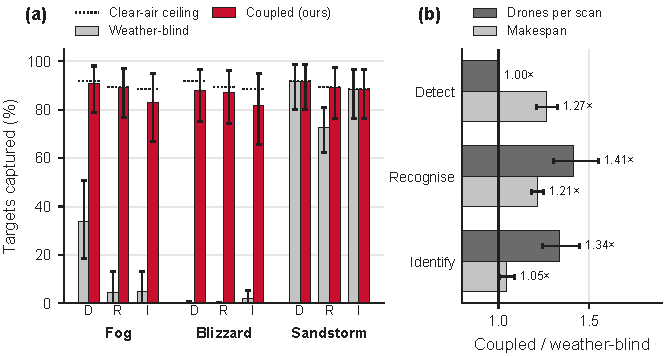
\includegraphics[width=\textwidth]{figures/pdf/coverage_eval.pdf}
\caption{Scan planning in low visibility, 7 cities and 3 seeds per preset. (a) Targets captured at the required level
(D detection, R recognition, I identification) by the weather-blind and the coupled plan; dotted lines are the
clear-air capture of the same tasks. (b) Drones per scan and makespan of the coupled plan relative to the blind plan,
over the feasible plans in the three presets}
\label{fig:coverage-eval}
\end{figure}

\paragraph{Task delegation.} Observation requests (a standing person to be detected, recognised or identified) are
delegated to a heterogeneous fleet: half the drones carry a zoom camera and half a fixed wide lens, and their states of
charge range from 12\% to 90\%, as between sorties. Every candidate quotes a request against the shared models: the
energy of the flight out at a corridor-safe altitude, a 60\,s observation and the flight home under the field wind,
and the perception level reached from the best of eight viewpoints around the target, with line of sight and slant
optical depth. Figure~\ref{fig:delegation} compares three awards on the same requests. Awarding the nearest drone, as
a distance-only dispatcher does, completes 42.2\% of requests. Of all its awards (one per request), 34.1\% break the launch reserve, among them
16.2\% that would strand the drone, and 35.8\% send a drone beyond the wind rating (the two overlap in strong wind); and a wide-lens drone is often nearest when a zoom
is needed. A contract net whose perception quote ignores line of sight and the atmosphere never breaks the reserve but
completes only 47.3\%, because it picks drones that cannot resolve the target. The contract net on the shared models
completes 58.6\% of requests, 94.2\% in clear air, never breaks the reserve, and declines the 37.8\% that no drone can
serve safely, mostly in thunderstorms, blizzards and sandstorms. The price is a 10\% longer time to the target (106\,s
against 96\,s), because the best drone is not always the nearest.

\begin{figure}[t]
\centering
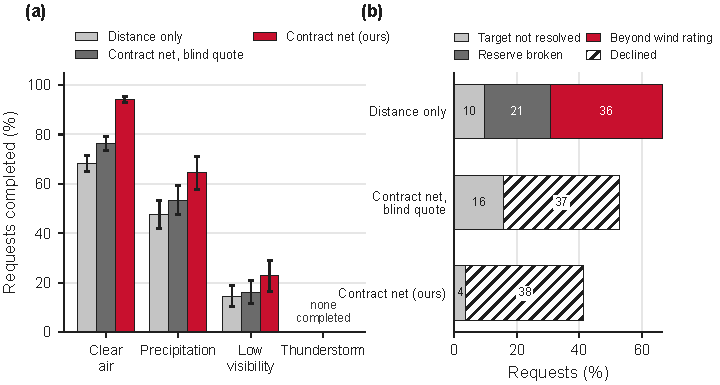
\includegraphics[width=\textwidth]{figures/pdf/delegation.pdf}
\caption{Capability-based delegation, 7 cities, 12 presets, 5 seeds, 30 requests each (12,600 requests per policy).
(a) Requests completed per weather group. (b) Why requests fail: the awarded drone cannot resolve the target, the
flight breaks the launch reserve, the route exceeds the wind rating, or the request is declined because no drone can
serve it}
\label{fig:delegation}
\end{figure}


\subsection{Ablation}\label{sec:eval:ablation}

Figure~\ref{fig:ablation} removes one coupling at a time from the coupled policy, on the same sorties. Each variant
turns off one decision-visibility switch of Sect.~\ref{sec:design:awareness} (\texttt{geometry}, \texttt{detour},
\texttt{wind}, \texttt{shared\_energy}, \texttt{energy\_rtl}) or the precheck; ``w/o detour'' is the
climb-to-clear return, which flies over the highest point of the envelope on the return line.
\begin{itemize}
\item \textbf{Geometry} is responsible for the safety of the return: without the corridor term, \NGCOLL\% of sorties
collide, and the share completed falls from \CPDONE\% to \NGDONE\%. The energy per completed sortie drops, but only because
the completed sorties are the short, low ones.
\item \textbf{Wind in the precheck} is responsible for launch safety: a wind-blind precheck launches more sorties and
completes more (\NWDONE\%), but \NWUNSAFE\% of all sorties become unsafe, mostly by launching beyond the rating in severe
weather.
\item \textbf{The shared energy model} is responsible for productivity: when the return trigger uses its own time-based
headwind model, \NSABORT\% of sorties are recalled early (against \CPABORT\%), the share completed falls to \NSDONE\%, and
completed sorties use \NSWHPCT\% more energy because recalled drones re-fly their transit. Safety is unchanged; this is the
model disagreement of F2, measured in closed loop.
\item \textbf{Detours} save climb and energy (Fig.~\ref{fig:overall-outcomes}b) and add \NDGAIN{} points of completed sorties.
\item \textbf{The energy-based trigger} matters only at the margin: with fixed battery thresholds alone, \NESTRAND\% of
sorties strand, against none.
\item \textbf{The precheck as a whole}: without it, every sortie launches; \NPUNSAFE\% are unsafe.
\end{itemize}
No single coupling delivers both safety and productivity; geometry, field wind and the shared energy model each remove a
different failure.

\begin{figure}[t]
\centering
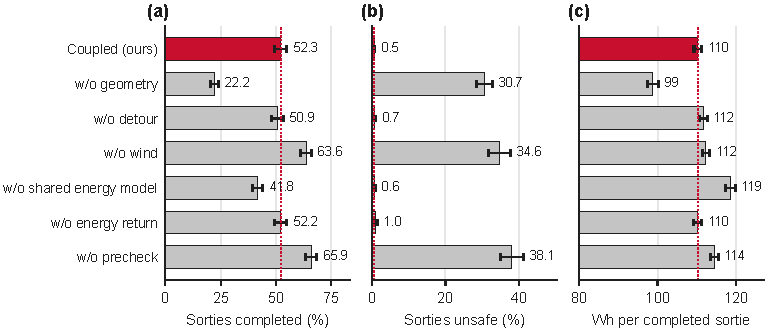
\includegraphics[width=\textwidth]{figures/pdf/ablation.pdf}
\caption{Ablation over all cities and presets (\RTLSORTIESPOL{} sorties per variant). (a) Sorties completed, (b)
sorties unsafe (lost or launched beyond the wind rating), (c) energy per completed sortie. Dotted lines mark the
coupled policy; bars show 95\% task-level bootstrap intervals}
\label{fig:ablation}
\end{figure}

\subsection{Cost of coupling}\label{sec:eval:micro}

All timings in this section come from one process pinned to one core of the server while nothing else runs; each value
is the median of seven timed calls after a warm-up, and the median over three repetitions.

\paragraph{Queries.} Batching is what makes shared models cheap (Fig.~\ref{fig:micro-queries}). A single surface-height
lookup costs 21.8\,$\mu$s, almost all of it call overhead; in batches of 10,000 it costs 0.01\,$\mu$s per point. The
corridor top along a return line, the query F1 needs, costs 63.6\,$\mu$s per line with an exact cell traversal and
0.61\,$\mu$s per line on the max-pooled height pyramid in batches of 1,000, a factor of 104. A line-of-sight test costs
9.8\,$\mu$s per pair in the maximal batch of 64. The environment field shows the same pattern: a wind query costs
27.8\,$\mu$s when issued point by point and 0.16\,$\mu$s per point in a batch of 10,000, and a slant optical depth
0.04\,$\mu$s per path. Evaluating all fields at once costs only a quarter more than wind alone, so a decision that
needs wind, visibility and density pays for one query, not three.

\begin{figure}[t]
\centering
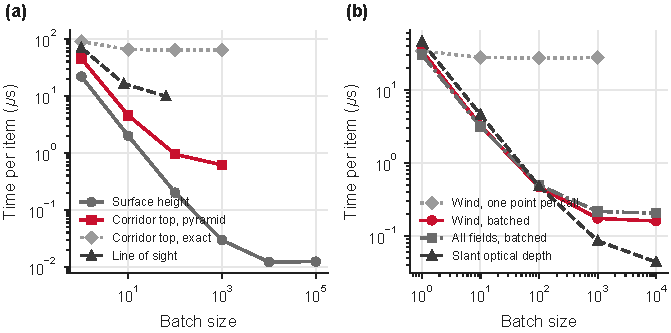
\includegraphics[width=\textwidth]{figures/pdf/micro_queries.pdf}
\caption{Query cost per item against batch size. (a) Geometry service: surface height, corridor top along a line (exact
traversal and pyramid sampling) and line of sight. (b) Environment field: wind one point per call and batched, all
fields batched, and slant optical depth}
\label{fig:micro-queries}
\end{figure}

\paragraph{Return refresh.} The rotating schedule turns the impossible schedule of F4 into a negligible one
(Fig.~\ref{fig:m4}). At 1,000 drones each 5\,Hz call refreshes 200 plans in 0.25\,ms, which amounts to 1.25
core-milliseconds per simulated second, against 3.1 for refreshing every drone at 5\,Hz, 153 for refreshing every drone
at every tick and 13,400 for doing so with exact corridors. The cost grows by a factor of 1.7 from 10 to 1,000 drones
because the fixed per-call overhead dominates; it stays below the 2 core-milliseconds the return stage is budgeted.
Plans are at most one second old, which at 3--8\,m/s is 3--8\,m of travel, well inside the 10\,m safety margin of the
clearance envelope.

\paragraph{Whole pipeline.} Figure~\ref{fig:micro-stages} runs the complete runtime with $N$ drones in rain, nearly
all flying, for 20 simulated seconds: environment, dynamics and control, sensors, contact and separation, the safety
state machines with the battery and return logic, missions and state publication, at the 4\,ms tick; scan planning and
delegation are invoked on demand and timed separately below. On a single core the runtime advances 1,000 drones at \STAGERTF{} times real time, so
real time needs \STAGECORE{} core-seconds per simulated second, inside the 0.40 budget; with 10 drones it runs
\STAGERTFTEN{} times faster than real time. Of the \STGTOT{} core-milliseconds the stages use per simulated second at
1,000 drones (\STGWALL{} including the loop around them), safety and energy take \STGSAFE{}, dynamics and control
\STGDYN{}, missions \STGMIS{}, the environment \STGENV{} and state publication \STGPUB{}. The environment stage grows
only from \STGENVTEN{} to \STGENV{} core-milliseconds between 10 and 1,000 drones, because one batched query serves
the whole fleet; the coupled decisions are thus not what limits the fleet size.

\begin{figure}[t]
\centering
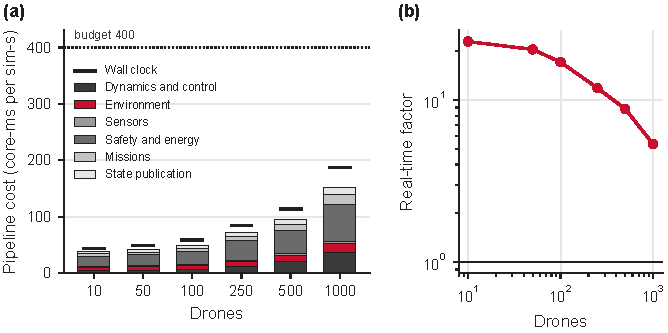
\includegraphics[width=\textwidth]{figures/pdf/micro_stages.pdf}
\caption{Whole pipeline with $N$ drones flying in rain, one core. (a) CPU cost per simulated second by stage group;
the dotted line is the 0.40 core-second budget. (b) Real-time factor (simulated seconds per wall-clock second)}
\label{fig:micro-stages}
\end{figure}

% \paragraph{Scan planner.} The perception-driven scan planner of Sect.~\ref{sec:design:decisions} plans a 0.04\,km$^2$
% area in 0.3\,s and a 4\,km$^2$ area in 2.0--2.4\,s (Fig.~\ref{fig:micro-coverage}), roughly linear in area. Planning therefore takes
% seconds, while the scans it plans take tens of minutes, and it can be rerun whenever the weather changes.

% \begin{figure}[t]
% \centering
% 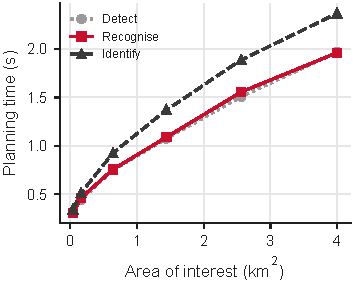
\includegraphics[width=0.55\textwidth]{figures/pdf/micro_coverage.pdf}
% \caption{Scan-planner runtime against the area of interest, per required perception level; median of three
% repetitions}
% \label{fig:micro-coverage}
% \end{figure}


\subsection{Access from ordinary devices}\label{sec:eval:access}

The server never renders; every view is drawn by the client from the streamed octree. We replay the same scripted
60\,s camera flight over Shenzhen (5.0 million points, $1600\times900$ viewport, three repetitions) on three clients:
headless Chromium with an NVIDIA A100 on the server's local network, Chrome on an Apple M3 laptop streaming from the
server over the public internet, and Chromium with the SwiftShader software renderer, a stand-in for a device
without a usable GPU. The client reports its own frame intervals, the points it draws and the screen-space error it
achieves. We compare the adaptive budget (APH with CAS) against fixed point budgets of 100k, 1M (the Potree
default~\cite{schuetz2020octree}) and 3M points (Fig.~\ref{fig:stream}).

No fixed budget is right for every device. On both GPU clients every budget reaches the display rate (16.7\,ms per
frame), and the adaptive controller raises its budget to the top of its ladder: it draws as many points as the 3M
budget and reaches the same screen-space error, below one pixel (Fig.~\ref{fig:stream}b), whereas 100k points leave a
median error of 10--14\,px. On the software renderer the picture reverses. With 1M or 3M points it renders at 12\,fps,
with a median frame time of 67--83\,ms and 83--85\% of frames beyond 1.5 times its 33.3\,ms target. The adaptive
controller holds the target (95th-percentile frame time 33.3\,ms, no frame beyond 1.5 times the target) and still draws
1.5 times as many points as the 100k budget, with a lower error (6.7 against 9.2\,px). Point selection costs at most
0.4\,ms per frame (95th percentile) on every client; slowing the M3's CPU four-fold by emulation changes neither its
frame times nor its error. The first view appears 1--2\,s after opening the page on the local network and after 14\,s
over the internet, where the 1.5\,MB first screen and the 22\,MB streamed during the flight compete with the path's
bandwidth. Because the server only serves static byte ranges and all selection runs in the client, adding viewers
adds file traffic but no per-viewer computation on the server; we did not measure many concurrent viewers.

\begin{figure}[t]
\centering
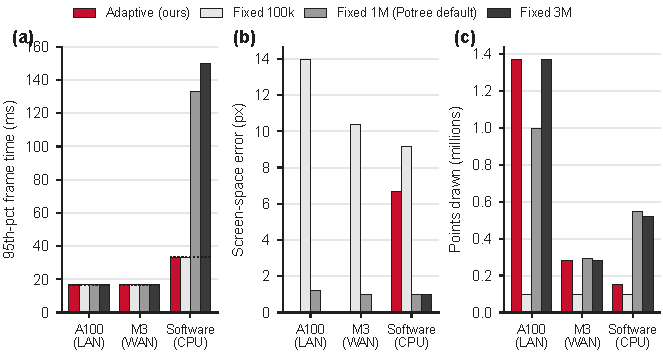
\includegraphics[width=\textwidth]{figures/pdf/stream.pdf}
\caption{The same 60\,s camera flight over Shenzhen on three clients, adaptive budget vs fixed budgets; medians of three
runs. (a) 95th-percentile frame time, with each client's frame target dotted. (b) Median screen-space error of the drawn
view. (c) Median number of points drawn}
\label{fig:stream}
\end{figure}


\subsection{Sensitivity}\label{sec:eval:sens}

Figure~\ref{fig:sens} varies the two decision parameters of the return and the visibility the scan planner faces. The
return sweeps run the coupled policy on three cities (Shenzhen, New York, SynthCity), clear weather and rain, three
seeds and all 25 combinations of the two margins; every combination flies the same sorties.

\paragraph{Clearance margin.} The margin above the corridor top trades launches for headroom
(Fig.~\ref{fig:sens}a). No setting from 0 to 20\,m lets a drone touch a building, because the clearance envelope
already contains a 10\,m safety margin and a 4\,m dilation. Larger margins raise the cruise and return altitudes,
which costs energy: at 20\,m the precheck declines 38.2\% of sorties instead of 27.1\% at the default of 5\,m, and
completion falls from 59.0\% to 50.7\%. Below 5\,m the gain is at most 1.4 points. The only contact in the sweep at a
margin of 0\,m is between two drones whose transit and return paths then coincide; inter-drone separation is handled by
the runtime's separation guard, not by the return planner.

\paragraph{Trigger margin.} The return starts when the remaining flight time falls below a multiple of the
energy-equivalent return time. Between 1.0 and 1.5 the outcome does not change (Fig.~\ref{fig:sens}b): with the shared
energy model the trigger is rarely the binding constraint, because the precheck has already budgeted the return. At 1.8
it recalls 16.7\% of sorties early instead of 13.9\% and completes 4.2 points fewer. The default of 1.3 sits in the flat
region, so the result does not depend on tuning it.

\paragraph{Visibility.} The coupled scan planner keeps capture within a few points of the clear-air ceiling down to a
MOR of about 200\,m (Fig.~\ref{fig:sens}c), where the weather-blind plan has already lost almost every target
(Fig.~\ref{fig:m3}a). It pays with drones: a recognition scan needs 1.76 drones on average in clear air, 2.29 at
200\,m and 3.19 at 100\,m. At 100\,m capture drops to 51--74\%, and 19--43\% of the plans are declined because no
lens resolves the target from a height that clears the buildings; the planner reports this before launch. The wind
sweep of Fig.~\ref{fig:m2} gives the corresponding sensitivity of launch and return to wind speed.

\begin{figure}[t]
\centering
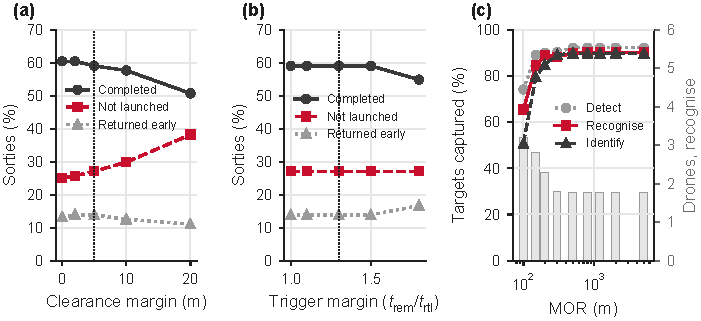
\includegraphics[width=\textwidth]{figures/pdf/sensitivity.pdf}
\caption{Sensitivity of the coupled policy. (a) Clearance margin above the corridor top and (b) return-trigger margin,
on the same 216 sorties per setting in clear weather and rain; dotted lines mark the defaults. (c) Scan planning under
a MOR sweep: targets captured at each level (lines, left axis) and drones a recognition scan needs (bars, right axis)}
\label{fig:sens}
\end{figure}


\subsection{Consistency and reproducibility}\label{sec:eval:consistency}

The design promises one model evaluated identically by the planner, the runtime and the display, and runs that are a
deterministic function of their seed. Table~\ref{tab:consistency} tests both. For the environment field we evaluate the
browser implementation on the golden vectors produced by the server implementation, over every function the display
uses. Of 79,104 outputs, 98.7\% are bit-identical and the largest absolute difference is $3.6\times10^{-12}$, from
floating-point reassociation in the wind composition; these differences are about ten orders of magnitude below the resolution of any decision threshold
(centimetres, tenths of a metre per second) and below single-precision rendering. For the fleet
runtime we run 18 configurations (three cities, clear, fog and thunderstorm weather, two seeds) three times each in
separate processes, with 16 drones flying for 180\,s in gusty wind, and hash the full fleet state every simulated
second. All 3,240 checkpoints agree across the three runs.

% generated by paper/figures/gen_numbers.py
\begin{table}[t]
\caption{Consistency of the shared environment model between the server and the browser, and replay determinism of the fleet runtime.}\label{tab:consistency}
\footnotesize
\begin{tabular*}{\textwidth}{@{\extracolsep{\fill}}lrrr@{}}
\toprule
Environment function & Outputs & Bit-identical & Max.\ abs.\ difference \\
\midrule
Field evaluation (wind, gust, optics) & 28,350 & 99.5\% & $3.6\times10^{-12}$ \\
Derived weather quantities & 19,228 & 99.9\% & $1.8\times10^{-15}$ \\
Wind sectors and slots & 17,352 & 100.0\% & 0 \\
Frame and unit conventions & 10,324 & 91.7\% & $5.7\times10^{-14}$ \\
Gust events & 1,837 & 99.9\% & $2.8\times10^{-16}$ \\
Slant optical depth & 687 & 93.4\% & $7.1\times10^{-15}$ \\
Turbulence box & 612 & 100.0\% & 0 \\
Standard atmosphere & 360 & 100.0\% & 0 \\
Keyframe anchors & 252 & 99.2\% & $6.7\times10^{-16}$ \\
Vertical wind profile & 102 & 100.0\% & 0 \\
\emph{All environment functions} & 79,104 & 98.7\% & $3.6\times10^{-12}$ \\
\midrule
Fleet replay (state hash per second) & 3,240 & 100\% & 0 \\
\bottomrule
\end{tabular*}
\end{table}

